\chapter{Sprint 0 – Migration de Panoramix}

\section*{Introduction}
Après avoir analyser et spécifier les besoins globaux de notre client, nous détaillerons les différentes étapes effectuées durant ce premier sprint ayant pour objectif « la migration de notre application ».  Cette migration assure la possibilité d’intégrer la nouvelle partie dans Panoramix.\\
Nous commencerons, tout d’abord, par présenter le backlog du sprint suivi d’une analyse détaillée et une comparaison entre les outils.

\section[Sprint Backlog]{Sprint Backlog}
Le tableau \ref{tab:sprint-backlog-sprint0}, qui représente une liste de tâches exprimées sous forme de besoins, illustre la liste des tâches de notre backlog de sprint
\begin{table}[H]
	\centering
	\begin{tabular}{|l|l|}
		\hline
		\rowcolor[HTML]{C0C0C0} 
		Exigences & Sous tâches                           \\ \hline
		1.1      & Migration de PHP 5.6 vers PHP 7.2    \\ \hline
		1.2      & Migration de MySQL vers MariaDB      \\ \hline
		1.3      & Migration de OFT2.2 vers OFT3        \\ \hline
		1.4      & Automatisation des tests de non régression \\ \hline
	\end{tabular}
	\captionsetup{justification=centering}
	\caption{Sprint backlog de sprint 0}
	\label{tab:sprint-backlog-sprint0}
\end{table}

\section[Migration de PHP 5.6 vers PHP 7.2]{Migration de PHP 5.6 vers PHP 7.2}
Dans cette section, nous comparons les critères le plus intéressants pour notre projet telque la performance, traitement des exceptions et le support de 64 bits entre les deux versions de PHP : version actuelle php5.3 et la version cible php7.2.

\subsection[Performance]{Performance}
Les performances de PHP 7 sont bien meilleures que celles de PHP 5. PHP 4 utilise le moteur Zend et PHP 5 utilise le moteur Zend II. Cependant, avec PHP 7, vient un tout nouveau moteur appelé PHPNG. Le "NG" signifie "Next Generation". Le moteur PHPNG améliore les performances du double avec une utilisation optimisée de la mémoire.
\begin{table}[H]
	\centering
	\begin{tabular}{l|l|l|}
		\cline{2-3}
		& \cellcolor[HTML]{C0C0C0}PHP5.3 & \cellcolor[HTML]{C0C0C0}PHP7.2 \\ \hline
		\multicolumn{1}{|l|}{\cellcolor[HTML]{C0C0C0}consommation de mémoire (Mo)}    & 7.8                            & 3.58 (-46\%)                   \\ \hline
		\multicolumn{1}{|l|}{\cellcolor[HTML]{C0C0C0}temps d'exécution CPU (seconde)} & 0.8                            & 0.35 (-44\%)                   \\ \hline
	\end{tabular}
\captionsetup{justification=centering}
	\caption{Comparaison de performance entre PHP 5.6 et PHP 7.2 sur le site journaldunet.com }
	\label{tab:perf-php}
\end{table}
\subsection[Traitement des exceptions]{Traitement des exceptions}
Le traitement des erreurs fatales dans le PHP 5 est assez compliqué. Le PHP 7 a remplacé plusieurs erreurs majeures avec des exceptions qui peuvent être traitées facilement. Cela est dû à l'introduction des nouveaux objets d'exception du moteur. 
\subsection[Support de 64 bits ]{Support de 64 bits }
PHP 5 ne prend pas en charge les entiers 64 bits ni les fichiers volumineux, alors que le PHP 7 supporte le 64 bits, ce qui permet d'utiliser des entiers 64 bits natifs et des fichiers volumineux.
\section[Migration de MySQL vers MariaDB]{Migration de MySQL vers MariaDB}
Dans cette partie du rapport, nous comparons le système de gestion de base de données actuel et le système de gestion de base de données cible. Nous examinerons les aspects liés aux performances, à la sécurité et aux principales caractéristiques, et nous énumérerons tous les aspects à prendre en compte avant de choisir la base de données qui répondra à nos besoins.
\subsection{Plus d'options pour les moteurs de stockage}
 y a 12 nouveaux moteurs de stockage intégrés dans MariaDB. Parmi ceux-ci, on trouve CONNECT, Spider et SphinxSE. Visitez leur page Moteurs de stockage pour une liste complète de ces moteurs, comment ils fonctionnent et comment les exploiter pour optimiser votre base de données.
\subsection{Améliorations de la vitesse}
MariaDB présente de nombreuses nouvelles améliorations de vitesse par rapport à MySQL standard. Ces performances améliorées permettent à MariaDB de se différencier des performances de base des serveurs MySQL traditionnels. Comme MySQL, MariaDB possède des dizaines de fonctionnalités pour l'optimisation de la vitesse, y compris l'accès au disque, les améliorations de JOIN et EXPLAIN, la sous-requête, les tables/vues dérivées, le contrôle de l'exécution et le contrôle de l'optimiseur.
\subsection{Indexes/Cache plus rapides}
En utilisant le moteur de stockage MEMORY, MariaDB peut compléter les instructions INSERT jusqu'à 24\% plus vite que les serveurs MySQL traditionnels, avec CHECKSUM TABLE et MyISAM Segment Key Cache étant 4x plus rapide.
\subsection{Un pool de connexion plus rapide et plus grand}
MariaDB bénéficie d'un pool de threads amélioré qui fonctionne plus rapide et prend en charge plus de 200 000 connexions là où MySQL standard ne supporte pas ce nombre.
\subsection{Réplication améliorée}
MariaDB bénéficie d'une réplication plus rapide et plus sûre, les mises à jour étant jusqu'à 2 fois plus rapides qu'avec les configurations de réplication MySQL traditionnelles. Désormais possible, la réplication parallèle assure l'existence de configurations Active/Active ou Master/Master. La réplication de MariaDB est rétrocompatible avec les serveurs MySQL, de sorte que la migration de votre cluster vers MariaDB est possible en utilisant un nœud à la fois.
\subsection{Nouvelles extensions/caractéristiques}
Il y a plusieurs nouvelles extensions et fonctionnalités, pour en nommer quelques-unes, les déclarations WITH, JSON et KILL. DECIMAL augmente de 30 à 38 décimales, tandis que KILL ALL permet d'effectuer des requêtes pour un utilisateur spécifique.
\subsection{Liste des fonctionnalités et la documentation}
Le site web MariaDB disponible présente une liste complète d'améliorations et de fonctionnalités, ainsi qu’une documentation bien détaillée.
\section{Migration d’OFT2 vers OFT3}
Dans cette section, nous présentons l’outil principal de développement de notre application OFT ( Orange Framework \& Tools ) et nous comparons les deux versions : version actuelle 2.2 et la version cible 3.
\subsection{Points forts d’OFT 3}
Parmi les principales raisons de migration, le support de PHP 7 d’où les versions précédentes  d’OFT ne sont pas compatibles avec PHP7. Un autre atout pour notre projet est la redirection simple des sorties des logs. En plus, les dépendances du framework ont été mises à jour et la performance de la framework est améliorée comme l'illustre la figure suivante :
\begin{figure}[H]
	\centering
	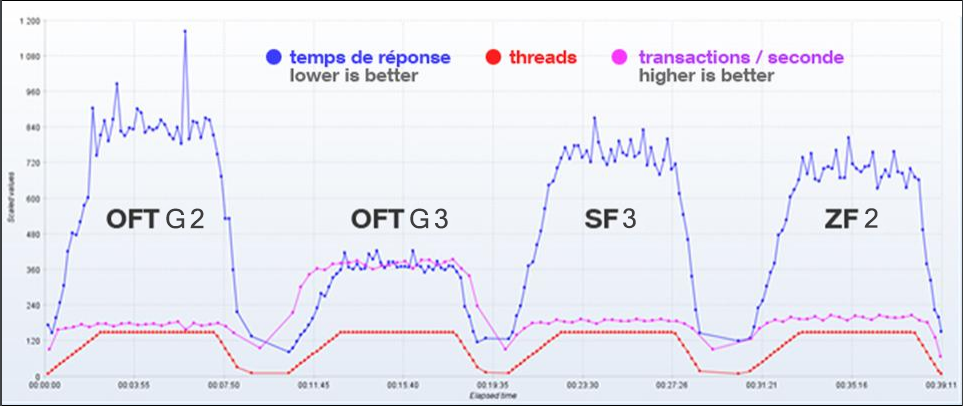
\includegraphics[width=0.7\linewidth]{img/oft-3}
	\caption[Comparaison performance entre OFT2 et OFT3]{Comparaison performance entre OFT2 et OFT3}
	\label{fig:oft-3}
\end{figure}
\section[Automatisation des tests de non régression]{Automatisation des tests de non régression}
Dans cette section, nous présentons la réalisation des différentes étapes d’automatisation des tests de non régression indiquées dans la figure \ref{fig:jenkins-schema} ci-dessus.
\subsection{Objectifs des tests}
Notre application Panoramix est considérée comme un portail qui assure l’accès aux différents PEFs ( points d’entrée fonctionnels ). Pour cela, l’équipe Panoramix décide de développer des  tests de non régression ou autrement des tests de l’IHM sur l’application de serveur d'intégration pour vérifier l’accès aux PEFs avec d’intégrer les modifications de code dans le serveur de production.
\subsection{Objectifs des tests}
Notre application Panoramix est considérée comme un portail qui assure l’accès aux différents PEFs ( points d’entrée fonctionnels ). Pour cela, l’équipe Panoramix décide de développer des  tests de non régression ou autrement des tests de l’IHM sur l’application de serveur d'intégration pour vérifier l’accès aux PEFs avec d’intégrer les modifications de code dans le serveur de production.
\subsection{Définition des tests}
Les tests sont envoyés sous format un fichier Excel contient :
\begin{itemize}
	\item Code de test : indique l’identifiant de chaque test
	\item fonctionnalité : indique une courte description de test
	\item jeu de données : cette colonne contient les valeurs de variables à utiliser
	\item Cas de gestion : précise la motif lors le test
	\item Etapes : représentent le scénario d'exécution de test
	\item Résultat attendu : précise le résultat de l’IHM après l'exécution de notre scénario  
	\item Ecrans : Capture d’écran de résultat attendu 
	\item Commentaire : Cette colonne est réservée aux commentaires supplémentaires ou une indication.
\end{itemize}
Nos 54 tests peuvent être présentés comme illustre la figure suivante :
\begin{figure}[H]
	\centering
	\includegraphics[width=1\linewidth]{"img/excel robot"}
	\caption[Fichier de description des tests]{Fichier de description des tests}
	\label{fig:excel-robot}
\end{figure}
\subsection{Réalisation}
Lors de cette partie, nous présenterons les différentes étapes de réalisation en spécifiant les étapes de configuration de Jenkins.\newpage
\subsubsection{Création de projet Jenkins}
Commençant tout d’abord par la création d’un projet Jenkins
\begin{figure}[H]
	\centering
	\includegraphics[width=0.9\linewidth]{"img/jenkins/creation projet"}
	\caption[Création de projet Jenkins]{Création de projet Jenkins}
	\label{fig:creation-projet}
\end{figure}

\subsubsection{Configuration du plugins}
Le projet est maintenant prêt, nous préparons les configurations nécessaires pour l'exécution des tests Cases de Robot Framework tels que les configurations du plugins :
\begin{itemize}
	\item \textbf{Xvfb plugin }
	\begin{figure}[H]
		\centering
		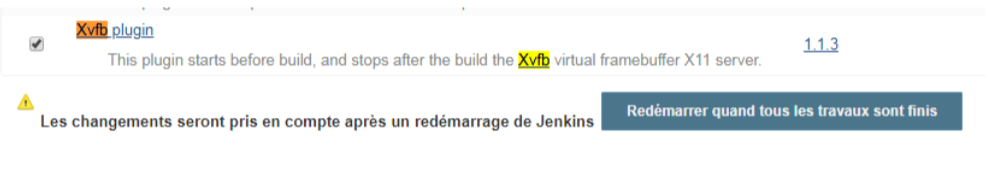
\includegraphics[width=0.9\linewidth]{img/jenkins/xvfb}
		\caption[plugin Xvfb]{plugin Xvfb}
		\label{fig:xvfb}
	\end{figure}
	
	\item \textbf{Email Extension}
	\begin{figure}[H]
		\centering
		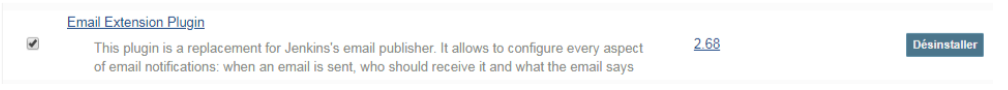
\includegraphics[width=0.9\linewidth]{img/jenkins/email}
		\caption[Email Extension plugin]{Email Extension plugin}
		\label{fig:email}
	\end{figure}
	
\end{itemize}
\newpage
et la configuration de l'environnement de build :
\begin{itemize}
	\item GeckoDrive
	\item Firefox
	\item Robot Framework
\end{itemize}
\begin{figure}[H]
	\centering
	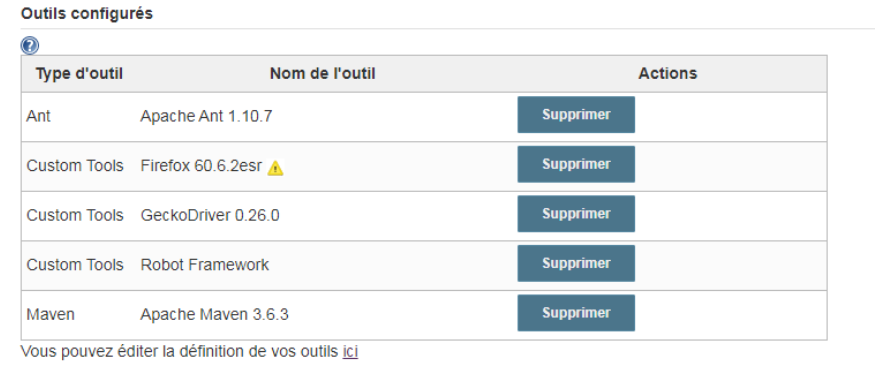
\includegraphics[width=0.7\linewidth]{img/jenkins/env-build}
	\caption[La configuration de l'environnement de build]{La configuration de l'environnement de build}
	\label{fig:env-build}
\end{figure}
\subsection{Gestion de code source}
Dans cette partie, nous configurons Jenkins de façon à récupérer les tests cases de Robot Framework. Nous choisissons la gestion de code avec Git et nous déclarons les dépôts distants hébergé chez Orange Forge avec la branche /develop. Chaque projet Jenkins possède un dépôt distant pour importer les tests. Lorsque le job est exécuté, Jenkins s’assure à chaque fois d’importer la dernière version des tests. Pour la configuration, il suffit de renseigner l’URL https de dépôts distants et fournir le nom d’utilisateur et le mot de passe. Un champ nous permet aussi de spécifier la branche du dépôt à utiliser comme l'illustre la figure suivante
\begin{figure}[H]
	\centering
	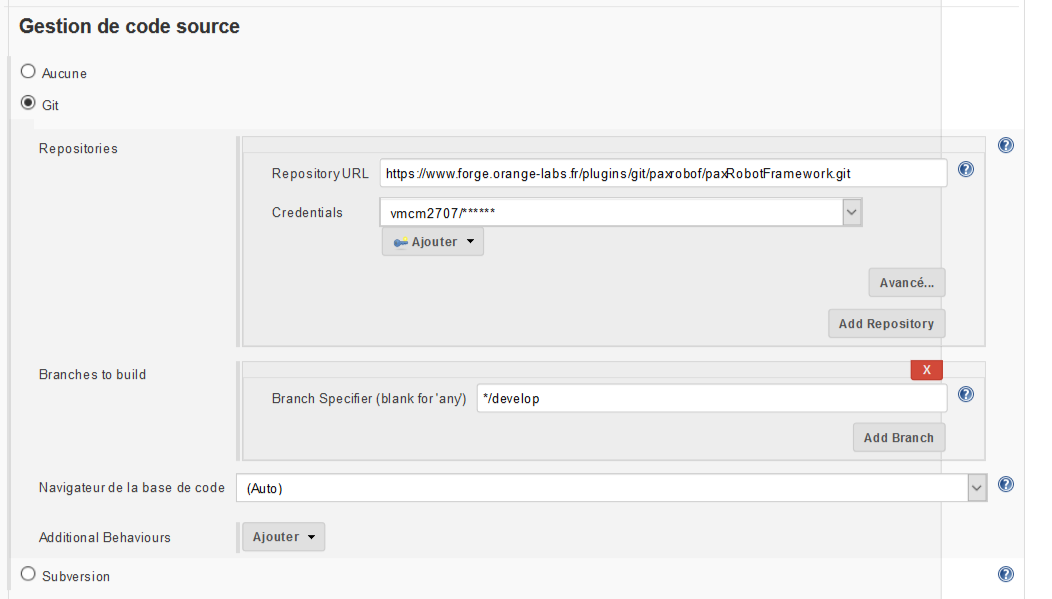
\includegraphics[width=0.7\linewidth]{img/jenkins/source}
	\caption[Gestion de source sous Jenkins]{Gestion de source sous Jenkins}
	\label{fig:source-jenkins}
\end{figure}

\subsection{Déclenchement de build }
Dans cette étape nous configurons la façon avec laquelle le job est lancé, plusieurs choix sont disponibles : soit périodiquement, soit par un déclencheur manuel.\\
Pour le premier choix, nous configurons la section “Ce qui déclenche le build” dans la configuration de job pour assurer que le build s'exécute de lundi à vendredi à 07:30 du matin.
\begin{figure}[H]
	\centering
	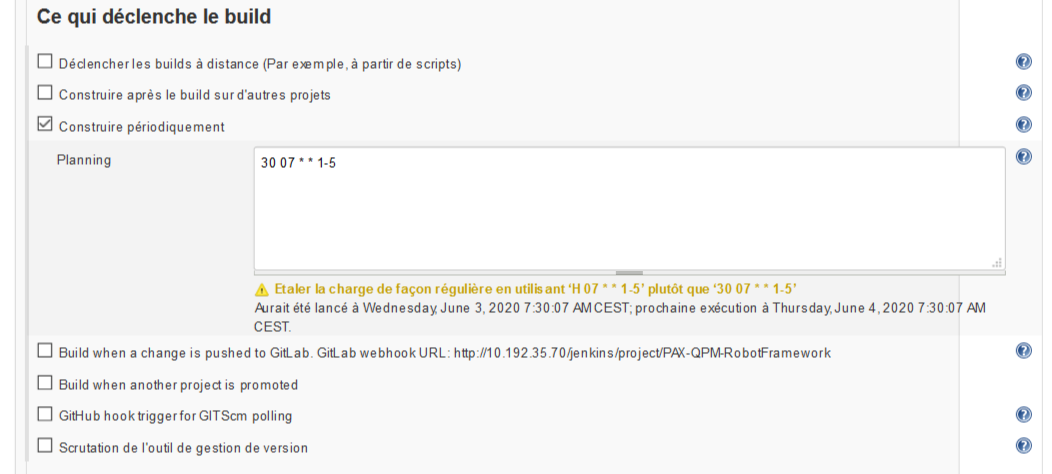
\includegraphics[width=0.8\linewidth]{img/jenkins/declanchement}
	\caption[Déclanchement de job Jenkins]{Déclanchement de job Jenkins}
	\label{fig:declanchement}
\end{figure}

\subsection{L’environnement de build}
\subsubsection{Build}
Dans cette étape, nous précisons l’action principale du job. Pour le job de tests, nous invoquons robot framework pour exécuter tous les tests cases dans le repo. Jenkins nous offre la possibilité de spécifier le chemin du test ainsi que le fichier robot. La figure présente notre configuration de déploiement.
\begin{figure}[H]
	\centering
	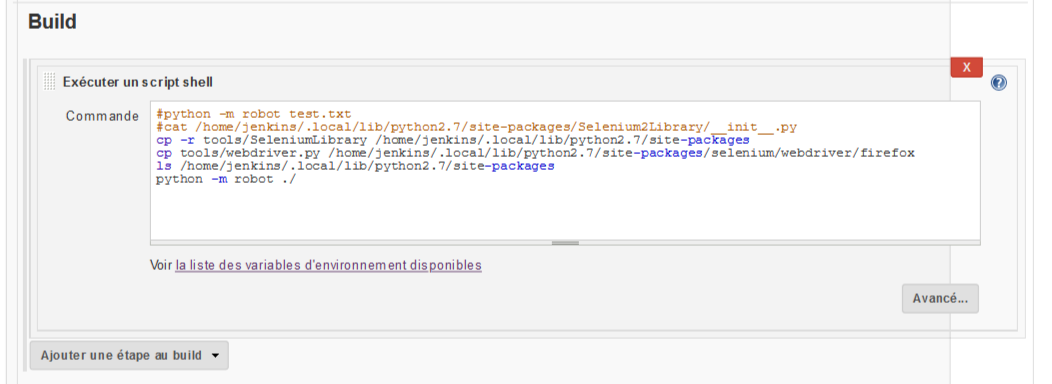
\includegraphics[width=0.8\linewidth]{img/jenkins/build}
	\caption[Build de job Jenkins]{Build de job Jenkins}
	\label{fig:build}
\end{figure}

\subsubsection{Actions à la suite du build}
Dans cette étape, nous activons la notification par mail, en attachant les  deux fichiers report.html et log.html, présenté par la figure suivante :
\begin{figure}[H]
	\centering
	\includegraphics[width=1\linewidth]{"img/jenkins/actions after"}
	\caption[Actions à la suite du build de job Jenkins]{Actions à la suite du build de job Jenkins}
	\label{fig:actions-after}
\end{figure}
\newpage
\subsection{Exécution de job}
Dans cette partie, nous présentons l’exécution du job. Jenkins offre la possibilité d’avoir une sortie console pour les commandes qu’il exécute.\\
La figure suivante représente la sortie de tous les outils du pipeline, ceci permet de garder une trace de l’exécution du job.
\begin{figure}[H]
	\centering
	\includegraphics[width=1\linewidth]{"img/jenkins/exemple console"}
	\caption[Extrait de sortie de console]{Extrait de sortie de console}
	\label{fig:exemple-console}
\end{figure}
l’exécution de robot framework génère deux fichiers qui résument les résultats de tests en basant sur des éléments graphiques facilitant la compréhension et la navigation.
\begin{itemize}
	\item Fichier report.html
	\begin{figure}[H]
		\centering
		\includegraphics[width=0.55\linewidth]{"img/jenkins/exemple report"}
		\caption[Extrait de rapport Jenkins]{Extrait de rapport Jenkins}
		\label{fig:exemple-report}
	\end{figure}
	\item Fichier log.html
	\begin{figure}[H]
		\centering
		\includegraphics[width=0.55\linewidth]{"img/jenkins/exemple log"}
		\caption[Extrait de log Jenkins]{Extrait de log Jenkins}
		\label{fig:exemple-log}
	\end{figure}
\end{itemize}

\section*{Conclusion}
Dans ce chapitre de sprint 0, nous avons migré notre application vers l’environnement souhaité et nous avons développé les tests et nous avons automatisé les tests sur jenkins.Dans le chapitre suivant, nous entamons de terminer la release 1 avec le sprint 1.



